%%%%%%%%%%%%%%%%%%%%%%%%%%%%%%%%%%%%%%%%%
% Short Sectioned Assignment
% LaTeX Template
% Version 1.0 (5/5/12)
%
% This template has been downloaded from:
% http://www.LaTeXTemplates.com
%
% Original author:
% Frits Wenneker (http://www.howtotex.com)
%
% License:
% CC BY-NC-SA 3.0 (http://creativecommons.org/licenses/by-nc-sa/3.0/)
%
%%%%%%%%%%%%%%%%%%%%%%%%%%%%%%%%%%%%%%%%%

%----------------------------------------------------------------------------------------
%	PACKAGES AND OTHER DOCUMENT CONFIGURATIONS
%----------------------------------------------------------------------------------------

\documentclass[paper=a4, fontsize=11pt]{scrartcl} % A4 paper and 11pt font size

\usepackage[T1]{fontenc} % Use 8-bit encoding that has 256 glyphs
\usepackage{fourier} % Use the Adobe Utopia font for the document - comment this line to return to the LaTeX default
\usepackage[spanish]{babel} % English language/hyphenation
\selectlanguage{spanish}
\usepackage[utf8]{inputenc}
\usepackage{amsmath,amsfonts,amsthm} % Math packages
\usepackage{graphicx}

\usepackage{sectsty} % Allows customizing section commands
\allsectionsfont{\centering \normalfont\scshape} % Make all sections centered, the default font and small caps

\usepackage{fancyhdr} % Custom headers and footers
\pagestyle{fancyplain} % Makes all pages in the document conform to the custom headers and footers
\date{}
\fancyhead{} % No page header - if you want one, create it in the same way as the footers below
\fancyfoot[L]{} % Empty left footer
\fancyfoot[C]{} % Empty center footer
\fancyfoot[R]{\thepage} % Page numbering for right footer
\renewcommand{\headrulewidth}{0pt} % Remove header underlines
\renewcommand{\footrulewidth}{0pt} % Remove footer underlines
\setlength{\headheight}{5.6pt} % Customize the height of the header

\numberwithin{equation}{section} % Number equations within sections (i.e. 1.1, 1.2, 2.1, 2.2 instead of 1, 2, 3, 4)
\numberwithin{figure}{section} % Number figures within sections (i.e. 1.1, 1.2, 2.1, 2.2 instead of 1, 2, 3, 4)
\numberwithin{table}{section} % Number tables within sections (i.e. 1.1, 1.2, 2.1, 2.2 instead of 1, 2, 3, 4)

\setlength\parindent{0pt} % Removes all indentation from paragraphs - comment this line for an assignment with lots of text

%----------------------------------------------------------------------------------------
%	TITLE SECTION
%----------------------------------------------------------------------------------------

\newcommand{\horrule}[1]{\rule{\linewidth}{#1}} % Create horizontal rule command with 1 argument of height

\title{	
\normalfont \normalsize 
\textsc{UNIVERSIDAD DE CANTABRIA, DEPARTAMENTO DE FÍSICA MODERNA} \\ [20pt] % Your university, school and/or department name(s)
\horrule{0.5pt} \\[0.4cm] % Thin top horizontal rule
\huge Física de Partículas Elementales (G71) \\ % The assignment title
\normalsize 4 Curso - Grado de Física - Primer parcial
\horrule{2pt} \\[0.5cm] % Thick bottom horizontal rule
}

\begin{document}

\maketitle % Print the title

\vspace{-2.5cm}

%----------------------------------------------------------------------------------------
%	PROBLEM 1
%----------------------------------------------------------------------------------------
\textbf{Cuestión 1.} Una de las reacciones posibles en el detector de neutrinos Superkamiokande es aquella en la que un 
neutrino interacciona con un neutrón de la piscina del detector dando lugar a un muon, un pion y otro neutrón $\nu + n\rightarrow\mu + \pi + n$.
Calcula la energía mínima del neutrino para que esta reacción sea posible. Considera: $m(\nu)\simeq 0~GeV$, $m(n)= 0.94~GeV$, $m(\mu) = 0.106~GeV$ y $m(\pi) = 0.140~GeV$. \textbf{(1 punto)}.
En la reacción anterior el pion y el neutrón se generan a través del decaimiento de un neutrón excitado intermedio $N^{\star}\rightarrow\pi + n$. ¿Cuál debe ser la masa mínima
del neutrón excitado para que sea posible dicho proceso?. \textbf{(1 punto)}. 
\\
\\
%----------------------------------------------------------------------------------------
%       PROBLEM 2
%----------------------------------------------------------------------------------------
\textbf{Cuestión 2.} Escribir la expresión de la regla de oro de Fermi y discutir el significado de los diferentes términos \textbf{(1 punto)}. Considera el proceso weak $e^{-}\nu_\mu\rightarrow\nu_e\mu^{-}$: dibuja el diagrama de Feynman asociado de primer orden \textbf{(0.5 puntos)}. Con ayuda de las reglas de Feynmann indica la estructura que tendría el elemento de matriz asociado, explicando brevemente lo que es cada término \textbf{(0.5 puntos)}.
%----------
\\
\\
%----------------------------------------------------------------------------------------
%       PROBLEM 3
%----------------------------------------------------------------------------------------
\textbf{Cuestión 3.} Prueba las siguientes relaciones de las matrices $\gamma$ en donde $a^\mu$ y $b^\mu$ son cuadrivectores cualesquiera. \textbf{(2 Puntos)}: 
\begin{enumerate}
\item $\gamma^\mu\gamma^\nu\gamma_\mu=-2\gamma^\nu$
\item $\gamma^\mu\gamma^\nu\gamma^\rho\gamma_\mu = 4g^{\nu\rho}$
\item $\gamma^\mu a_\nu \gamma^{\nu}\gamma_\mu = -2a_\nu\gamma^{\nu}$
\item $\gamma^\mu a_\nu \gamma^{\nu} b_\rho \gamma^{\rho} \gamma_\mu = 2 a^{\mu}b_\mu$
\end{enumerate}
%----------------------------------------------------------------------------------------
%       PROBLEM 4
%----------------------------------------------------------------------------------------
\textbf{Cuestión 4.} Utilizando la expresión $(\gamma^\mu p_\mu - m)u = 0$ obten la expresión para el spinor adjunto $\bar{u}(\gamma^\mu p_\mu - m) = 0$ sabiendo que $\{\gamma^\mu, \gamma^\nu\}=2g^{\mu\nu}$ \textbf{(1 punto)}. Sin utilizar las expresiones explíticas para los espinores $u$, muestra que si tenemos la condición de normalización $u^\dag u=2E$, entonces $\bar{u}u = 2m$ \textbf{(1 punto)}. \textbf{Pista:} Multiplica $\bar{u}\gamma^\nu$ por la izquierda a $(\gamma^\mu p_\mu - m)u = 0$ y $\gamma^\nu u$ por la derecha a $\bar{u}(\gamma^\mu p_\mu - m) = 0$, súmalas y considera el caso $\nu=0$ sabiendo que $(\gamma^0)^2=1$.
%----------------------------------------------------------------------------------------
\\
\\
%----------------------------------------------------------------------------------------
%       PROBLEM 5
%----------------------------------------------------------------------------------------
\textbf{Cuestión 5.} Definir el concepto de helicidad. \textbf{(0.5 Puntos)}. ¿Por qué se dice que el momento angular orbital no es una buena magnitud para estudiar las soluciones de la ecuación de Dirac? \textbf{(0.5 Puntos)}.
\\
\\
%----------------------------------------------------------------------------------------
%       PROBLEM 6
%----------------------------------------------------------------------------------------
\textbf{Cuestión 6.} ¿A qué llamamos operador conjugación de carga y cómo se relaciona con la interacción electromagnética?. Demuestra que si aplicamos el operador conjugación de carga
a los espinores de partícula en \ref{espinores}, obtenemos los espinores de antipartícula. \textbf{(1 Punto)}.
\\
\\

\begin{figure}[!h]
\begin{center}
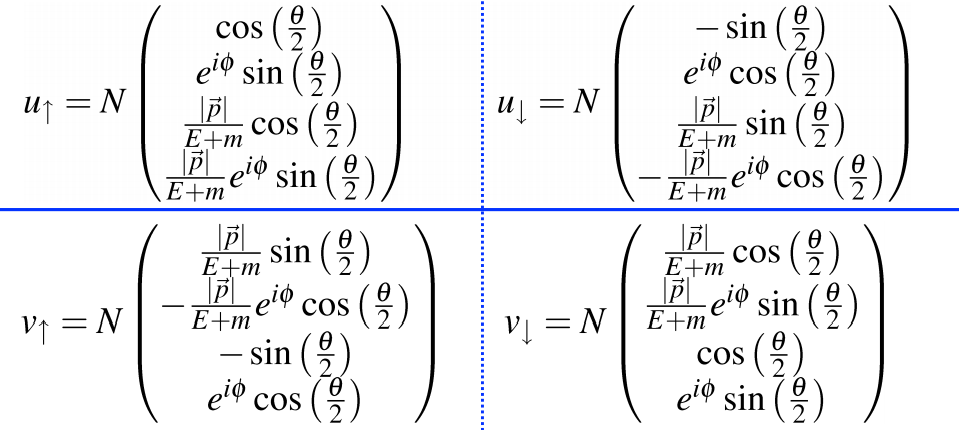
\includegraphics[width=0.6\linewidth]{espinores.png}
\end{center}
\caption{Espinores solución a la ecuación de Dirac y autoestados del operador helicidad.}
\label{espinores}
\end{figure}


\begin{figure}[!h]
\begin{center}
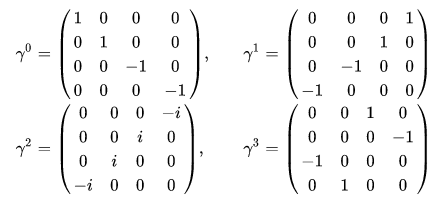
\includegraphics[width=0.6\linewidth]{matrices.png}
\end{center}
\caption{Matrices de Dirac.}
\label{matrices}
\end{figure}






\end{document}
